\chapter{Introducción}
\label{sec:introduction}

La elaboración de pan comprende una secuencia de operaciones que incluye
la preparación y dosificación de ingredientes, el mezclado, la división
y formado de la masa, la fermentación y la cocción, con variaciones según
el tipo de producto y el método empleado
\parencite{cauvain2015technology}. Dentro de esta secuencia, la
dosificación establece las cantidades de ingredientes que serán
incorporadas a cada preparación antes del mezclado.

La Panadería San Miguel, ubicada en Santa Cruz de la Sierra, constituye
el caso de estudio del presente proyecto. Durante el relevamiento de
campo se documentaron preparaciones de pan casero, marraqueta y pan
francés en una jornada ordinaria. En la jornada de sábado se registró
una preparación de pan casero y una masa común destinada posteriormente
a empanadas y rollos de queso. Para efectos del proyecto, el análisis se
concentra exclusivamente en la dosificación de harina de trigo previa al
mezclado y amasado.

La Figura~\ref{fig:proceso_general_pan} presenta las principales etapas
del proceso de elaboración del pan y permite identificar la etapa de
dosificación de harina comprendida dentro del alcance del presente
proyecto.

\begin{figure}[htb]
    \centering

    \resizebox{0.95\textwidth}{!}{%
        {\setlength{\fboxsep}{10pt}
        \fbox{%
            \begin{tikzpicture}[
    node distance=8mm and 8mm,
    >=Latex,
    block/.style={
        rectangle,
        draw,
        minimum height=1.2cm,
        text width=3.2cm,
        align=center,
        font=\small
    },
    alcance/.style={
        block,
        dashed,
        very thick,
        font=\small\bfseries
    },
    arrow/.style={
        -{Latex[width=8pt,length=6pt]},
        thick
    }
]

% -----------------------------------------------------------------
% Primera fila
% -----------------------------------------------------------------

\node (preparacion) [block]
{Preparación de\\ingredientes};

\node (dosificacion) [alcance, right=of preparacion]
{Dosificación de\\ingredientes\\
\textit{\footnotesize Alcance: harina}};

\node (mezclado) [block, right=of dosificacion]
{Mezclado y\\amasado};

\node (formado) [block, right=of mezclado]
{División y\\formado};


% -----------------------------------------------------------------
% Segunda fila
% -----------------------------------------------------------------

\node (fermentacion) [block, below=12mm of formado]
{Fermentación};

\node (horneado) [block, left=of fermentacion]
{Horneado};

\node (producto) [block, left=of horneado]
{Producto\\terminado};


% -----------------------------------------------------------------
% Conexiones
% -----------------------------------------------------------------

\draw [arrow] (preparacion) -- (dosificacion);
\draw [arrow] (dosificacion) -- (mezclado);
\draw [arrow] (mezclado) -- (formado);

\draw [arrow]
    (formado.south)
    -- ++(0,-5mm)
    -| (fermentacion.north);

\draw [arrow] (fermentacion) -- (horneado);
\draw [arrow] (horneado) -- (producto);

\end{tikzpicture}
        }}
    }

    \caption{Proceso general de elaboración del pan.}
    \label{fig:proceso_general_pan}

    \vspace{0.2em}
    {\footnotesize Fuente: Elaboración propia.}

\end{figure}

La dosificación de harina se encuentra ubicada antes de la etapa de
mezclado y amasado. El alcance del proyecto se limita a esta operación,
por tanto, las etapas posteriores del proceso productivo no forman parte
del desarrollo principal del sistema propuesto.

La dosificación gravimétrica automatizada ha sido estudiada como una
alternativa para suministrar ingredientes a partir de una cantidad
objetivo previamente definida. En aplicaciones de panificación se han desarrollado sistemas que
integran mecanismos de alimentación, celdas de carga y estrategias de
control para dosificar harina y otros ingredientes
\parencite{farihin2021premix,humaira2024optimalisasi}. Asimismo, se han
reportado desarrollos orientados específicamente a la dosificación
automática de harina para pequeñas y medianas panaderías
\parencite{rumapea2026flour}.

Estos antecedentes muestran la aplicabilidad de sistemas de dosificación
gravimétrica en procesos de panificación. Sin embargo, la selección y el
diseño de una solución para la Panadería San Miguel deben considerar las
cantidades de harina utilizadas, la secuencia de trabajo, las
características del material, la distribución del área y las condiciones
reales de operación del establecimiento.

En este contexto, el presente proyecto se orienta al desarrollo de un
prototipo automatizado de dosificación gravimétrica de harina para la
Panadería San Miguel. El estudio comprende la caracterización del
procedimiento manual, el establecimiento de requerimientos, el diseño e
integración del prototipo y la evaluación de su desempeño frente al
procedimiento actual.


%%%%%%%%%%%%%%%%%%%%%%%%%%%%%%%%%%%%%%%%%%%%%%%%%%%%%%%%%%%%%%%%%%%%%%%%%%%%%%%
% PLANTEAMIENTO DEL PROBLEMA
%%%%%%%%%%%%%%%%%%%%%%%%%%%%%%%%%%%%%%%%%%%%%%%%%%%%%%%%%%%%%%%%%%%%%%%%%%%%%%%

\section{Planteamiento del Problema}
\label{sec:problema}

\subsection{Antecedentes del Problema}
\label{subsec:antecedentes_problema}

Para caracterizar el procedimiento actual de dosificación de harina se
realizó un levantamiento de campo en la Panadería San Miguel. El área
relacionada con esta operación comprende la zona de almacenamiento de
harina, la mesa donde se encuentra instalada la balanza y la amasadora.
La disposición de estos elementos se encuentra condicionada por los
accesos existentes, la ubicación del suministro de agua y la organización
del área de producción.

Durante el levantamiento se registró una distancia de
$3{,}20\ \mathrm{m}$ por trayecto entre la zona de almacenamiento de
harina y el punto de pesaje. La Figura~\ref{fig:croquis_panaderia}
presenta la distribución del área vinculada con la dosificación e
identifica los principales elementos que intervienen en el recorrido
realizado por el operario.

\begin{figure}[htb]
    \centering
    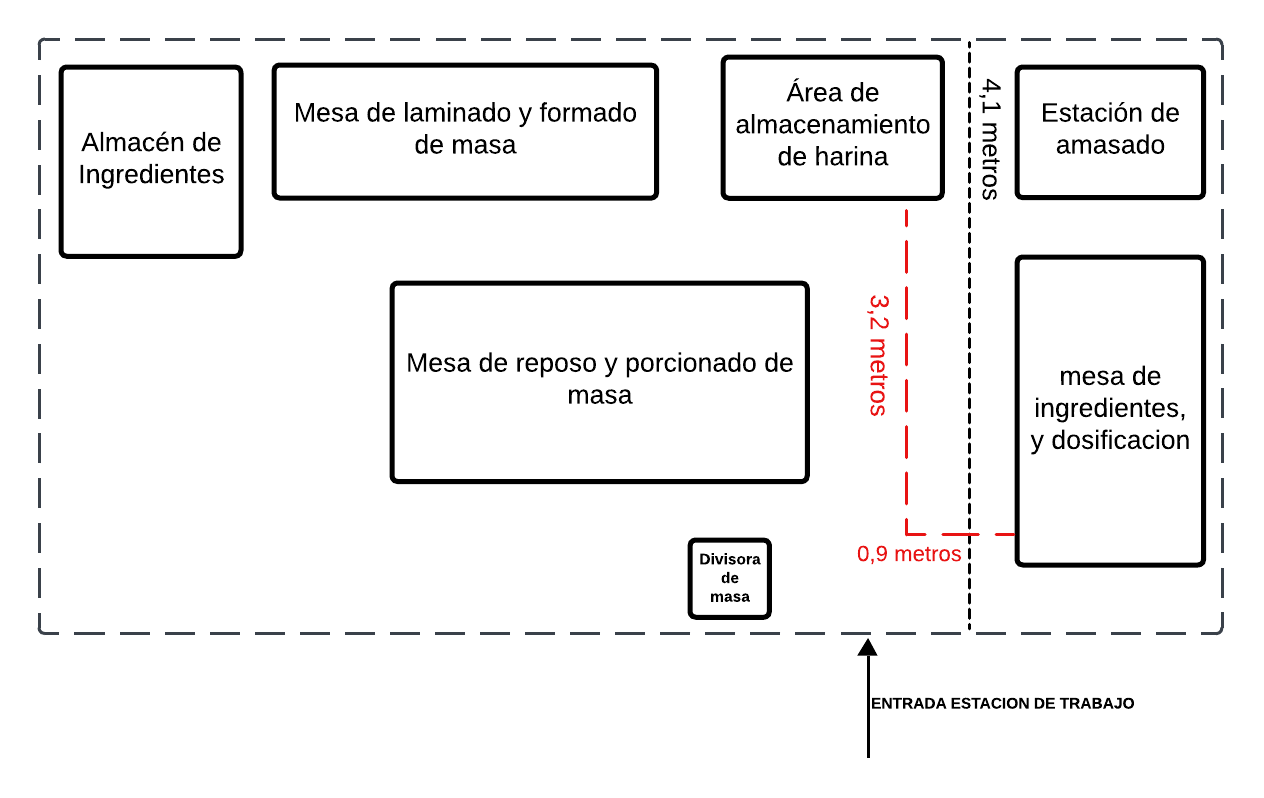
\includegraphics[width=0.95\textwidth]{images/marcoref/croquis_panaderia.png}
    \caption{Distribución del área relacionada con la dosificación de harina en la Panadería San Miguel.}
    \footnotesize{Fuente: Elaboración propia.}
    \label{fig:croquis_panaderia}
\end{figure}

El procedimiento observado inicia con la preparación del recipiente
receptor sobre la balanza, seguida de la aplicación de la función de
tara y la comprobación de la indicación de cero. Posteriormente, el
operario se desplaza hacia la zona de almacenamiento de harina, recoge
una carga mediante un recipiente de transporte, retorna al punto de
pesaje y descarga el contenido en el recipiente receptor.

Cuando la cantidad de harina acumulada permanece por debajo de la cantidad
establecida para la receta, el operario retorna a la zona de almacenamiento
para recoger una carga adicional y repite la operación. Después de la última carga
principal se realiza un ajuste final empleando la harina remanente en el
recipiente de transporte. Finalmente, se comprueba la lectura indicada por
la balanza y el recipiente de transporte es devuelto a la zona de harina.

Para describir de manera sistemática el ciclo de dosificación se
identificaron las siguientes actividades: preparación y tara (P),
desplazamiento inicial hacia la zona de harina (I), recogida, traslado y
descarga de una carga principal (C), retorno para realizar una carga
adicional (R), ajuste final y comprobación de la lectura (F), y devolución
del recipiente de transporte (D).

La función de tara se realiza una sola vez por ciclo. Asimismo, el ajuste
final no requiere un trayecto adicional hacia la zona de almacenamiento,
debido a que se efectúa utilizando la harina remanente de la última carga
transportada.

La Figura~\ref{fig:dfd_dosificacion} representa la secuencia de
actividades que conforman el procedimiento manual actual de dosificación
de harina. En ella se identifican las etapas de preparación, pesaje,
carga, verificación de la cantidad de harina acumulada, repetición de
cargas cuando corresponde y finalización del ciclo.

\begin{figure}[H]
    \centering
    \resizebox{0.8\textwidth}{!}{
        {\setlength{\fboxsep}{14pt}
        \fbox{\begin{tikzpicture}[
    >=Latex,
    proceso/.style={
        rectangle,
        draw,
        rounded corners=2pt,
        minimum width=4.3cm,
        minimum height=1.1cm,
        text width=3.9cm,
        align=center,
        font=\small
    },
    decision/.style={
        diamond,
        draw,
        aspect=2.2,
        text width=3.0cm,
        align=center,
        inner sep=1.2pt,
        font=\small
    },
    iniciofin/.style={
        rectangle,
        draw,
        rounded corners=12pt,
        minimum width=2.8cm,
        minimum height=0.8cm,
        align=center,
        font=\small
    },
    flecha/.style={
        -{Latex[width=7pt,length=6pt]},
        thick
    }
]

% ================================================================
% COLUMNA IZQUIERDA
% ================================================================

\node (inicio) [iniciofin] at (0,0)
{Inicio};

\node (preparar) [proceso] at (0,-1.7)
{Preparar recipiente de dosificación};

\node (tara) [proceso] at (0,-3.6)
{Colocar el balde en la balanza, aplicar TARE y verificar cero};

\node (nuevacarga) [proceso] at (0,-7.1)
{Agregar harina};

\node (volver) [proceso] at (0,-5.4)
{Volver a pesar};

% ================================================================
% COLUMNA DERECHA
% ================================================================

\node (carga) [proceso] at (6.8,-3.6)
{Recoger, trasladar y descargar harina en el recipiente receptor};

\node (medir) [proceso] at (6.8,-5.4)
{Medir masa acumulada};

\node (decision) [decision] at (6.8,-7.6)
{¿Se requiere otra carga?};

\node (finalizar) [proceso] at (6.8,-10.0)
{Realizar ajuste final, comprobar la lectura y finalizar la dosificación};

\node (fin) [iniciofin] at (6.8,-11.7)
{Fin};

% ================================================================
% FLUJO PRINCIPAL
% ================================================================

\draw[flecha] (inicio) -- (preparar);
\draw[flecha] (preparar) -- (tara);
\draw[flecha] (tara.east) -- (carga.west);
\draw[flecha] (carga) -- (medir);
\draw[flecha] (medir) -- (decision);

\draw[flecha]
    (decision.south) -- node[right,font=\small] {No} (finalizar.north);

\draw[flecha] (finalizar) -- (fin);

% ================================================================
% BUCLE DE REPETICIÓN
% ================================================================

\draw[flecha]
    (decision.west) -- ++(-1.2,0)
    node[above,font=\small,pos=0.35] {Sí}
    -- (nuevacarga.east);

\draw[flecha] (nuevacarga.north) -- (volver.south);
\draw[flecha] (volver.east) -- (medir.west);

\end{tikzpicture}}}}
    \caption{Diagrama de flujo del procedimiento manual actual de dosificación de harina.}
    \footnotesize{Fuente: Elaboración Propia.}
    \label{fig:dfd_dosificacion}
\end{figure}

El intervalo utilizado para el análisis comienza con la preparación del
recipiente receptor y concluye una vez comprobada la lectura final y
devuelto el recipiente de transporte. El abastecimiento y apertura de
una nueva bolsa de harina, el traslado posterior hacia la amasadora y
las operaciones posteriores de elaboración del producto quedan fuera de
este intervalo.

La evidencia consolidada comprende siete ciclos de dosificación
correspondientes a dos jornadas de observación. La jornada ordinaria,
registrada el 2 de septiembre de 2026, comprende cinco ciclos de
dosificación: dos de pan casero, dos de marraqueta y uno de pan francés.
La jornada de sábado, registrada el 5 de septiembre de 2026, comprende
dos ciclos: uno de pan casero y uno correspondiente a una masa común
utilizada posteriormente para empanadas y rollos de queso.

Las lecturas acumuladas de la balanza y los registros de cantidad de
harina utilizados para el análisis se presentan en el
Apéndice~\ref{ap:registros_campo}, mientras que la desagregación de los
tiempos por actividad se incluye en el
Apéndice~\ref{ap:tablas_dosificacion}.

La Tabla~\ref{tab:resumen_dosificacion} presenta los resultados
consolidados de las jornadas registradas. La diferencia de cantidad de
harina se determina mediante:

\[
\Delta h = h_{\mathrm{final}} - h_{\mathrm{objetivo}},
\]

donde $h_{\mathrm{final}}$ corresponde a la cantidad final de harina
registrada y $h_{\mathrm{objetivo}}$ a la cantidad de harina establecida
para la receta.

\begin{table}[H]
    \centering
    \caption{Resumen de los ciclos de dosificación de harina registrados}
    \label{tab:resumen_dosificacion}
    \small

    \begin{tabular}{lccccc}
        \hline
        \textbf{Jornada} &
        \textbf{Ciclos} &
		\textbf{\shortstack{Harina de\\receta (kg)}} &
		\textbf{\shortstack{Harina\\final (kg)}} &
		\textbf{\shortstack{Diferencia de\\harina (kg)}} &
        \textbf{\shortstack{Tiempo\\(s)}} \\
        \hline

        Día de semana &
        5 &
        $36{,}500$ &
        $36{,}578$ &
        $+0{,}078$ &
        $304{,}5$ \\

        Sábado &
        2 &
        $11{,}500$ &
        $11{,}565$ &
        $+0{,}065$ &
        $107{,}4$ \\

		\textbf{Total} &
		\textbf{7} &
		$\mathbf{48{,}000}$ &
		$\mathbf{48{,}143}$ &
		$\mathbf{+0{,}143}$ &
		$\mathbf{411{,}9}$ \\

        \hline
    \end{tabular}

    \vspace{0.4em}

    \parbox{0.94\textwidth}
	\footnotesize{Fuente: Elaboración Propia.}
\end{table}


El tiempo acumulado para los cinco ciclos de la jornada ordinaria fue de
$304{,}5\ \mathrm{s}$, mientras que los dos ciclos de la jornada de
sábado sumaron $107{,}4\ \mathrm{s}$. En conjunto se registraron
$411{,}9\ \mathrm{s}$, equivalentes a $6\ \mathrm{min}$ y
$51{,}9\ \mathrm{s}$.

Los tiempos individuales se encontraron entre $53{,}2\ \mathrm{s}$ y
$66{,}6\ \mathrm{s}$. Estos valores cuantifican el tiempo destinado a la
operación de dosificación dentro de los límites definidos y no
constituyen, por sí solos, una medición de tiempo perdido ni del ahorro
que podría alcanzar una alternativa automatizada.

Las operaciones de recogida, traslado y descarga de cargas principales,
junto con los retornos requeridos para realizar cargas adicionales,
acumularon $259{,}7\ \mathrm{s}$ de los $411{,}9\ \mathrm{s}$
registrados, equivalentes al $63{,}0\%$ del tiempo total. Este valor
comprende tanto la manipulación de harina como el desplazamiento del
operario y, por tanto, no corresponde exclusivamente a tiempo de
caminata.

Respecto de la cantidad de harina dosificada, las lecturas finales de
los siete ciclos se encontraron por encima de las cantidades de harina
establecidas para las respectivas recetas.

Las diferencias individuales registradas variaron entre
$+0{,}011\ \mathrm{kg}$ y $+0{,}038\ \mathrm{kg}$, con una diferencia
acumulada de $+0{,}143\ \mathrm{kg}$. Estos resultados corresponden a
las jornadas observadas y no permiten establecer desperdicio,
incumplimiento de una tolerancia o alteraciones en la calidad del
producto. La definición de un criterio de aceptación requiere considerar
las características de las recetas, la resolución y las características
metrológicas del sistema de pesaje, además de los requerimientos
establecidos para el prototipo.

% PENDIENTE DE CAMPO:
% Registrar:
% - marca de la balanza,
% - modelo,
% - capacidad máxima,
% - división/resolución,
% - información disponible sobre precisión o verificación.

Para estimar la acumulación mensual del tiempo destinado a la
dosificación se considera el calendario de septiembre de 2026,
compuesto por 22 días de lunes a viernes y cuatro sábados. Bajo el
supuesto de repetición de las condiciones registradas para cada tipo de
jornada, el tiempo mensual proyectado se determina mediante:

\[
22(304{,}5\ \mathrm{s})
+
4(107{,}4\ \mathrm{s})
=
7\,128{,}6\ \mathrm{s}.
\]

El resultado equivale a $1\ \mathrm{h}$, $58\ \mathrm{min}$ y
$48{,}6\ \mathrm{s}$ de actividad de dosificación durante el mes. Esta
estimación se obtiene a partir de las jornadas observadas y no
representa una medición mensual directa. La proyección no incorpora
cierres, feriados, variaciones de producción ni modificaciones de las
condiciones registradas.

A partir de los tiempos registrados y de su acumulación en las jornadas
observadas, el tiempo de intervención directa del operario se establece
como la variable central del planteamiento.

\newpage

La Figura~\ref{fig:arbol_problemas} presenta la relación entre las
causas identificadas, la condición central del planteamiento y los
efectos temporales derivados de los registros y de la proyección
mensual.

\begin{figure}[H]
    \centering
    \resizebox{0.8\textwidth}{!}{
        \begin{minipage}{0.98\textwidth}
\centering

%%%%%%%%%%%%%%%%%%%%%%%%%%%%%%%%%%%%%%%%%%%%%%%%%%%%%%%%%%%%%%%%%%%%%%%%%%%%%%%
% EFECTOS
%%%%%%%%%%%%%%%%%%%%%%%%%%%%%%%%%%%%%%%%%%%%%%%%%%%%%%%%%%%%%%%%%%%%%%%%%%%%%%%

\textbf{EFECTOS OBSERVADOS Y PROYECTADOS}\\[0.5em]

\begin{tabular}{p{0.44\textwidth} p{0.44\textwidth}}

\fbox{\parbox{0.42\textwidth}{\centering
\textbf{E1}\\[0.3em]
Acumulación del tiempo destinado a la dosificación durante las jornadas
observadas\\[0.3em]
{\small
304,5 s en la jornada ordinaria\\
107,4 s en la jornada de sábado}
}}
&
\fbox{\parbox{0.42\textwidth}{\centering
\textbf{E2}\\[0.3em]
Acumulación mensual proyectada del tiempo destinado a la dosificación\\[0.3em]
{\small
7\,128,6 s para septiembre de 2026\\
1 h 58 min 48,6 s}
}}

\end{tabular}

\vspace{0.7em}

{\Large $\uparrow\qquad\qquad\qquad\uparrow$}

\vspace{0.7em}

%%%%%%%%%%%%%%%%%%%%%%%%%%%%%%%%%%%%%%%%%%%%%%%%%%%%%%%%%%%%%%%%%%%%%%%%%%%%%%%
% PROBLEMA CENTRAL
%%%%%%%%%%%%%%%%%%%%%%%%%%%%%%%%%%%%%%%%%%%%%%%%%%%%%%%%%%%%%%%%%%%%%%%%%%%%%%%

\fbox{\parbox{0.90\textwidth}{\centering
\textbf{PROBLEMA CENTRAL}\\[0.4em]

El procedimiento manual de dosificación de harina en la Panadería
San Miguel requiere intervención directa del operario durante
$53{,}2$--$66{,}6\ \mathrm{s}$ por ciclo.
}}

\vspace{0.7em}

{\Large $\uparrow\qquad\uparrow\qquad\uparrow$}

\vspace{0.7em}

%%%%%%%%%%%%%%%%%%%%%%%%%%%%%%%%%%%%%%%%%%%%%%%%%%%%%%%%%%%%%%%%%%%%%%%%%%%%%%%
% CAUSAS
%%%%%%%%%%%%%%%%%%%%%%%%%%%%%%%%%%%%%%%%%%%%%%%%%%%%%%%%%%%%%%%%%%%%%%%%%%%%%%%

\textbf{CAUSAS OBSERVADAS}\\[0.5em]

\begin{tabular}{p{0.30\textwidth} p{0.30\textwidth} p{0.30\textwidth}}

\fbox{\parbox{0.28\textwidth}{\centering
\textbf{C1}\\[0.3em]
Preparación del recipiente, aplicación de tara y comprobación de cero
en cada ciclo
}}
&
\fbox{\parbox{0.28\textwidth}{\centering
\textbf{C2}\\[0.3em]
Dosificación mediante cargas principales realizadas manualmente\\[0.3em]
{\small
3--4 cargas principales por ciclo}
}}
&
\fbox{\parbox{0.28\textwidth}{\centering
\textbf{C3}\\[0.3em]
Ajuste final y comprobación manual de la lectura de la balanza
}}

\end{tabular}

\end{minipage}
    }
    \caption{Árbol de problemas de la dosificación manual de harina en
    la Panadería San Miguel.}
    \label{fig:arbol_problemas}

    \vspace{0.2em}

    {\small Fuente: Elaboración propia.}
\end{figure}

La Tabla~\ref{tab:trazabilidad_arbol} relaciona los elementos
presentados en el árbol con la evidencia obtenida durante el
levantamiento de campo y con los valores calculados a partir de las
jornadas observadas.

\begin{table}[H]
    \centering
    \caption{Trazabilidad de los elementos del árbol de problemas}
    \label{tab:trazabilidad_arbol}
    \small

    \begin{tabularx}{\textwidth}{|l|X|X|}
        \hline

        \textbf{ID} &
        \textbf{Elemento} &
        \textbf{Evidencia disponible} \\
        \hline

        C1 &
        Preparación del recipiente, aplicación de tara y comprobación de cero
        en cada ciclo. &
        La actividad P se registró en los siete ciclos observados. \\
        \hline

        C2 &
        Dosificación mediante cargas principales realizadas manualmente. &
        Se registraron tres o cuatro cargas principales por ciclo y
        24 cargas principales en los siete ciclos observados. \\
        \hline

        C3 &
        Ajuste final y comprobación manual de la lectura. &
        La actividad F se registró en los siete ciclos observados. \\
        \hline

        E1 &
        Acumulación del tiempo destinado al procedimiento de dosificación
        durante las jornadas observadas. &
        Se registraron $304{,}5\ \mathrm{s}$ en los cinco ciclos de la
        jornada ordinaria y $107{,}4\ \mathrm{s}$ en los dos ciclos de la
        jornada de sábado. \\
        \hline

        E2 &
        Acumulación mensual proyectada del tiempo destinado a la
        dosificación. &
        La proyección para septiembre de 2026 corresponde a
        $7\,128{,}6\ \mathrm{s}$, equivalentes a
        $1\ \mathrm{h}$, $58\ \mathrm{min}$ y
        $48{,}6\ \mathrm{s}$. \\
        \hline

    \end{tabularx}

    \vspace{0.4em}

    {\footnotesize Fuente: Elaboración propia.}

\end{table}

La trazabilidad muestra que las causas C1, C2 y C3 corresponden a
actividades registradas durante los siete ciclos observados. El efecto
E1 reúne los tiempos acumulados de las dos jornadas, mientras que E2
corresponde a la proyección mensual calculada a partir de dichos
registros. En conjunto, la evidencia sustenta el tiempo de intervención
directa del operario como variable central del planteamiento.

%%%%%%%%%%%%%%%%%%%%%%%%%%%%%%%%%%%%%%%%%%%%%%%%%%%%%%%%%%%%%%%%%%%%%%%%%%%%%%%
% FORMULACIÓN DEL PROBLEMA
%%%%%%%%%%%%%%%%%%%%%%%%%%%%%%%%%%%%%%%%%%%%%%%%%%%%%%%%%%%%%%%%%%%%%%%%%%%%%%%

\subsection{Formulación del Problema}
\label{subsec:formulacion_problema}

Durante las jornadas observadas, el procedimiento manual de dosificación
de harina en la Panadería San Miguel requirió intervención directa del
operario durante $53{,}2$--$66{,}6\ \mathrm{s}$ por ciclo, con tiempos
acumulados de $304{,}5\ \mathrm{s}$ en la jornada ordinaria y
$107{,}4\ \mathrm{s}$ en la jornada de sábado.

%%%%%%%%%%%%%%%%%%%%%%%%%%%%%%%%%%%%%%%%%%%%%%%%%%%%%%%%%%%%%%%%%%%%%%%%%%%%%%%
% OBJETIVOS
%%%%%%%%%%%%%%%%%%%%%%%%%%%%%%%%%%%%%%%%%%%%%%%%%%%%%%%%%%%%%%%%%%%%%%%%%%%%%%%

\section{Objetivos}
\label{sec:objetivos}

\subsection{Objetivo General}
\label{subsec:objetivo_general}

Desarrollar un prototipo automatizado de dosificación gravimétrica de
harina para la Panadería San Miguel y evaluar su desempeño frente al
procedimiento manual en términos de tiempo por ciclo, diferencia
respecto de la cantidad objetivo de harina, repetibilidad e intervención
del operario.

\subsection{Objetivos Específicos}
\label{subsec:objetivos_especificos}

\begin{enumerate}

\item Caracterizar el procedimiento manual de dosificación de harina
mediante el relevamiento de una jornada ordinaria y una jornada de
sábado, cuantificando las cantidades objetivo y finales de harina, los
tiempos por ciclo, el número de cargas y la intervención del operario.

\item Establecer los requerimientos funcionales y técnicos del
prototipo a partir de las cantidades de harina utilizadas, las
condiciones del área, la secuencia del procedimiento y los criterios de
desempeño definidos para el sistema.

\item Diseñar los subsistemas mecánico, de medición gravimétrica y de
control del prototipo de acuerdo con los requerimientos establecidos.

\item Construir e integrar un prototipo funcional de dosificación
gravimétrica automatizada conforme al diseño desarrollado.

\item Evaluar el desempeño del prototipo bajo condiciones equivalentes
al procedimiento manual, comparando el tiempo por ciclo, la diferencia
absoluta respecto de la cantidad objetivo de harina, la repetibilidad y
la intervención requerida del operario.

\end{enumerate}